The problem of finding every center and angle of rotation of a fixed shape ellipse which makes it have three points on its border is presented in this section. Even though its simple statement--it is short and uses only basic mathematical concepts--we were not able to find any work on it, or even on related problems. 
As a result, starting from scratch, we ended up trying a handful of approaches with most of them failing on the way. We try to give a review of some of those, going through the issues with the failing ones. At the end we propose a $\bigO(1)$ algorithm that finds every solution of the problem, and also run some experiments to analyze efficiency in terms of numerical precision and CPU time.

We refer to this problem as \sigla{E3PNT}{Ellipse by Three points}, and an instance of it is given by three points $u, v, w \in \R^2$ and $E$, the coverage area of an ellipse with shape parameters $(a, b) \in \R^2_{>0}$, with $a > b$. A solution of E3PNT is a pair $(q, \theta) \in \R^2\times[0, \pi)$, such that $\{u, v, w\} \subset \partial E(q, \theta)$. Because of its application on \autoref{chapter:ellipses_n}, every solution of E3PNT must be encountered. This is a vital piece of information which makes this problem more challenging.

\section{Transforming the problem}

To make it simpler, let us translate the system, so the point $u$ is at $(0,0)$. Then, we assume that the ellipse is actually axis-parallel and the points are the ones rotating. When an angle is found such that the three points lie on the border of the axis-parallel ellipse, a linear transformation can be applied to compress the x-axis by $\frac{b}{a}$, transforming the ellipse into a circle of radius $b$. This transformation can be seen on \autoref{fig:circumscribed-circle} where a solution of the E3PNT is transformed into a solution of the problem of finding a circumscribed circle of a triangle. 
This process can be parametrized by the angle of rotation of the points, as described by \autoref{eq:trpnts}, and because of the invertibility of linear transformations, solutions for E3PNT can be obtained by reversing these transformations.

\begin{figure}
	\centering
	\caption{Transforming an ellipse into a circle. T1, T2, and T3 represent the steps of the transformation.}
	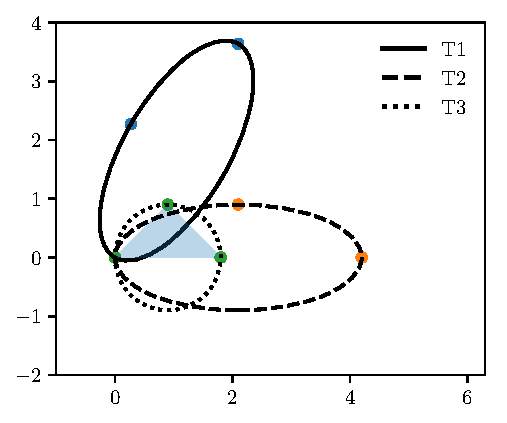
\includegraphics{tex/figures/scripts/circumscribed-circle}
	\fautor
	\label{fig:circumscribed-circle}
\end{figure}
\begin{equation}\label{eq:trpnts}
\varphi(p, \theta)=\left[\begin{array}{cc}
\frac{b}{a}&0\\
0&1
\end{array}\right]
\left[\begin{array}{cc}
\cos{\theta}&\sin{\theta}\\
-\sin{\theta}&\cos{\theta}
\end{array}\right]\left[\begin{array}{c}
p_x\\
p_y
\end{array}\right].
\end{equation}

After that transformation, the problem to be solved is finding a circumscribed circle of the triangle formed by the points $\{(0, 0), \varphi(v, \theta),\varphi(w, \theta)\}$, such that the circle's radius is $b$. Therefore, the only unknown of this problem is the angle of rotation. This idea reduces the number of variables from $3$ to only $1$, however, this would only be useful if checking the existence of a circumscribed circle with radius $b$ is a convenient problem.

It turns out that for three non-colinear fixed points, there is always an unique circumscribed circle. Also, finding this unique circle can be done analytically, hence its radius can be easily computed and compared to $b$ when an angle is given.
Let $A(\theta)$ be the area of the triangle formed by the points $\{(0, 0), \varphi(v, \theta), \varphi(w, \theta)\}$--note that the transformation does not preserve distance or area. Then, the radius $R$ of the circumscribed circle is given by \autoref{eq:circumscribed_circle} \cite[p.~189]{johnson1960}.

\begin{equation}\label{eq:circumscribed_circle}
R = \dfrac{\norm{\varphi(v, \theta)}\norm{\varphi(w, \theta)}\norm{\varphi(v, \theta)-\varphi(w, \theta)}   }{4A(\theta)}.
\end{equation}

Imposing the radius to be equal $b$ and squaring to eliminate the square roots present in the Euclidean distance, a function $\xi : [0, 2\pi) \mapsto \mathbb{R}_{>0}$ is defined by \autoref{eq:circumscribed_circle_b} in such a way that its zeros determine solutions to the E3PNT's instance. Two questions about $\xi(\theta)$ that arise are: is its set of roots finite? And, can they be found analytically?

\begin{equation}\label{eq:circumscribed_circle_b}
\xi(\theta) = 16b^2A(\theta)^2 - \norm{\varphi(v, \theta)}^2\norm{\varphi(w, \theta)}^2\norm{\varphi(v, \theta)-\varphi(w, \theta)}^2.
\end{equation}

\subsection{The number of solutions is limited}

One of the steps of the method developed on \autoref{chapter:ellipses_n} is to iterate over every solution of E3PNT for every triplet of points. Of course doing that is only possible for a finite number of solutions. Also, discovering a bound for that is essential for determining the efficiency of the algorithm.

Back on \autoref{chapter:definitions} real trigonometric polynomials were introduced. It was stated that a $n$-degree polynomial can have up to $2n$ distinct roots. It turns out that $\xi$ is a real trigonometric polynomial of degree $6$ and it can be written in the format given by \autoref{eq:trig_poly_2} which implies that it can have up to $12$ distinct roots.
 To show that, just note that it is possible to write $\norm{\varphi(v, \theta)}^2$ and $A(\theta)^2$ in that form, as it can be seen on \autoref{eq:dd} and \autoref{eq:dd2}. It is also possible to see that the term of higher the degree of $\xi$ is the multiplication of the three squared distances. As $\norm{\varphi(v, \theta)}^2$ has degree $2$, the degree of $\xi$ is $6$.
\begin{align}\label{eq:dd}
	\norm{\varphi(v, \theta)}^2 = (v_x\frac{b}{a}\cos\theta + v_y\frac{b}{a}\sin\theta)^2 + (v_y\cos\theta - v_x\sin\theta)^2\\
	\label{eq:dd2} A(\theta)^2=\dfrac{1}{4}\det\left(
	\begin{array}{cc}
		v_x\frac{b}{a}\cos\theta + v_y\frac{b}{a}\sin\theta&v_y\cos\theta - v_x\sin\theta\\
		w_x\frac{b}{a}\cos\theta + w_y\frac{b}{a}\sin\theta&w_y\cos\theta - w_x\sin\theta
	\end{array}\right)^2
\end{align}

Because ellipses are symmetrical with respect to their major-axis, and any rotation in the interval $[0, \pi)$ is identical to a rotation in $[\pi, 2\pi)$, the number of different solutions is cut in half.
Therefore, the number of angles of rotation and centers that an ellipse of fixed shape can be placed, so it has three fixed points on its border is limited to $6$.

\section{An attempt using the conic general equation}

The idea of this approach was to use the six-parameter conic equation to represent an ellipse. This equation is given by \autoref{eq:gen_ellipse}.

\begin{equation}\label{eq:gen_ellipse}
Ax^2+Bxy+Cy^2+Dy+Ex+F=0.
\end{equation}
This equation actually represents any conic, for it to be an ellipse the condition $B^2 -4AC < 0$ must be satisfied.

Setting the first point to be the origin, we get $F=0$, using the other two points, it is possible to write $D$ and $E$ in terms of $A, B, C$. As any multiple of \autoref{eq:gen_ellipse} represents the same conic, we can set $B$ to be equal $1$. Then, we end up with two variables, $A$ and $C$, and still need to impose that the final equation represents an ellipse and its major-axis and minor-axis have the predefined value. Let $\Delta=4AC-B^2=4AC-1$, \autoref{eq:gen_ellipse_a} and \autoref{eq:gen_ellipse_b} for both major-axis and minor-axis respectively, assuming $F=0$.

\begin{align}\label{eq:gen_ellipse_a}
a^2 = \dfrac{2\dfrac{AE^2 -BDE +CD^2}{\Delta}}{A + C - \sqrt{1 + (A-C)^2}}\\
\label{eq:gen_ellipse_b}b^2 = \frac{2\dfrac{AE^2 -BDE +CD^2}{\Delta}}{A + C + \sqrt{1 + (A-C)^2}}
\end{align}

These two equations define two curves in $\R^2$ with $A$ and $C$ being the chosen variables. The solutions lie in the set of intersection of these curves. Finding this set was judged to be non-trivial and probably could be approximated numerically, however, we decided not to further pursue this approach.

Another idea which has been explored was working with the ratio $\frac{a^2}{b^2}$ which becomes an expression that allows $A$ to be written as a function of $C$. This function appeared, at first we thought, to be monotonic, we tried to develop a method based on that, however, cases where the function does not behave as nicely were found. It is likely that developing a method to approximate solutions working with this function is possible, but we decided not to continue on this track.


\section{An approximation method}

One of the most useful techniques when dealing with complicated functions is approximation. They appear in various methods whenever a derivative or integral needs to be calculated or for example, in our case, when the roots of a function need to be determined. In general, one has a function $f$ that is part of a family of functions $\mathcal{A}$ and wants to select a simpler function $f^*$ from a set of functions $\mathcal{A^*}$, such that $f^*$ is close enough to $f$ \cite[p.~3]{powell}. For this problem, the approximation of $\xi(\theta)$ on the interval $[0, \pi)$ is considered. The approximation set of functions is going to be the set of $n$-degree Chebyshev polynomials which the roots can be found through determining the eigenvalues of a $n$ by $n$ matrix.


\subsection{Chebyshev interpolation}

Chebyshev polynomials are widely used in Numerical Analysis in areas like numerical integration, polynomial approximation, and ordinary and partial differential equations.
They are also very useful in practice and are present in extension libraries in Python and MATLAB.

Because of the scope of this work, only a brief introduction of Chebyshev polynomials of the first kind and its usage in polynomial interpolation is given. For a more thorough work on the subject, please check the book by \citeonline{chebbook}.

We refer to $T_n : [-1, 1] \mapsto [-1, 1]$ as the $n$-degree Chebyshev polynomial of the first kind, and it is defined as follows:

\begin{equation}
T_n(x) = \cos({n\arccos x})
\end{equation}

It is important to mention that this definition can be extended to the whole real line. Using some trigonometric identities, $T_n$ can also be expressed as a recurrence relation:

\begin{equation}
T_n(x) = 2xT_{n-1}(x) - T_{n-2}(x).
\end{equation}

An important property worth bringing up is that Chebyshev polynomials are orthogonal and form a basis for the polynomial space. This implies that any $p_n$ of degree up to $n$ can be expressed as a truncated Chebyshev series:

\begin{equation}\label{eq:chebseries}
p_n(x) = \sum_{j=0}^{n} a_j T_j(x).
\end{equation}

One of the greatest qualities of Chebyshev polynomials is its numerical stability. \citeonline{gautschi:1979} showed that the matrix that maps polynomials onto its coefficients written in the power form\footnote{A polynomial is in the power form or the monomial form if it can be written as $\sum_{j=0}^{n}a_jx^j$} has a condition number that grows exponentially with $n$. On the other hand, the matrix that converts polynomials to the Chebyshev basis as \autoref{eq:chebseries}, has a linear condition number bounded by $\sqrt{2}n$.

Polynomial interpolation is a form of approximating a function by a polynomial of degree $n$ that passes through $n+1$ chosen points. In fact, this polynomial is unique and it is determined by Lagrange's formula:

\begin{equation}\label{eq:lagrange}
f_n(x) = \sum_{j=0}^{n} f(x_j)\dfrac{\prod_{k \neq j}^{n+1} (x-x_k)}{\prod_{k \neq j}^{n+1} (x_j-x_k)},
\end{equation} 
with $f$ being the function to be approximated, and $f_n$ the unique $n$-degree polynomial that passes through $\{(x_j, f(x_j)): j=0, 1, \dots n\}$. Because of the uniqueness of interpolant polynomials, there is a direct link between the quality of an approximation and the points chosen to interpolate. As a matter of fact, depending on the points one chooses, even increasing the degree of the interpolation makes the approximation worsen. This is known as Runge's phenomenon and an example can be seen in \citeonline[p.~37]{powell} where uniformly spaced points are chosen to interpolate the function $f(x) = (1+x^2)^{-1}$ on the interval $[-5, 5]$. 

That is where Chebyshev interpolation comes in. Instead of choosing $n+1$ arbitrary points, the $n+1$ roots of $T_{n+1}$, which are also known as Chebyshev Nodes, are chosen as the interpolation points:
\begin{equation}
x_j = \cos{\left(\dfrac{\pi(k-\frac{1}{2})}{n+1}\right)},
\end{equation}
for $j=1, \dots, n+1$. This particular choice defeats Runge's phenomenon and provides a convergent approximation. 

Note that, if the domain of the function to be interpolated is defined on a range other than $[-1, 1]$, let us say $[a, b]$, then a transformation can be done to map it to the Chebyshev Nodes' domain:
\begin{equation}
\hat{x_j} = \frac{a+b}{2} + \frac{b-a}{2}x_j.
\end{equation}

Then, the Chebyshev interpolation of a function $f: [a, b] \mapsto \R$ can be determined using Lagrange's formula and the points $\hat{x}_1, \dots, \hat{x}_n$. 
As it was mentioned, finding the roots of a polynomial written in the monomial form can be done by determining the eigenvalues of a so-called Frobenius companion matrix. For small $n$ this works fine, however, converting the polynomial obtained by \autoref{eq:lagrange} to the power form, as $n$ grows, becomes a very ill-conditioned problem. 
An alternative method can be found in \citeonline{boyd:2013} where the Chebyshev interpolation is calculated directly as a truncated Chebyshev series, as in \autoref{eq:chebseries}, in $\bigO(n^2)$. Also, given a polynomial written in the Chebyshev basis, a $n\times n$ matrix can be constructed, such that its eigenvalues are the roots of that polynomial. \citeonline{boyd:2013} refers to this matrix as the Chebyshev-Frobenius companion matrix.

Therefore, the whole process of interpolating and finding the roots can be done using only Chebyshev polynomials, which have great numerical stability. Also, Chebyshev-Frobenius matrices have the same property as companion matrices which allows their eigenvalues to be found by a QR decomposition. Summing the two steps, a $\bigO(n^2)$ algorithm can be achieved.

The last question that needs to be addressed is how close the roots of the Chebyshev interpolant $f_n$ are to the roots of $\xi$?

Even though $\xi$ is complicated enough, in a sense that finding its roots directly is no trivial task, it is a very well-behaved function: it is analytic and  has infinitely many continuous and integrable derivatives. This satisfy all the requirements of the result in \citeonline[p.~28]{gottlieb} which says that if a function has $m$ continuous and integrable derivatives on a closed interval, then its absolute difference between the Chebyshev truncate series is $\bigO(n^{-m})$. Also, in \citeonline{battles:2004} a theorem is presented stating that if a function is analytic on a neighborhood of $[-1, 1]$, then the convergence is $\bigO(C^n)$, for some $C<1$.

To choose the degree of the interpolation we use the last coefficient rule-of-thumb introduced by \citeonline[p.~50]{boyd:2001}. There is no guarantee that this method will choose $n$, such that $f_n$ is close enough to $\xi$ everywhere on $[0, \pi)$, nonetheless, in practice, it is taken to be a good estimate for the error $r_n$:
\begin{equation}
r_n = \max_{0 \le \theta \le \pi} |f_n(\theta) - \xi(\theta)|.
\end{equation}


\section{Converting $\xi$ into a polynomial}

On \autoref{chapter:definitions} a brief introduction is given on how to get the roots of a polynomial. For that reason, we discuss two ways of converting $\xi$ into a polynomial in this section. Symbolic computing was used to compute the polynomials, the Python external library called SymPy was utilized (see \citeonline{sympy} for more details).

\subsection{Real polynomial}

The first attempt was using the identity $x = \tan{\frac{\theta}{2}}$ from which it is possible to construct a $12$-degree polynomial. At first,  the root-finding algorithm described on \autoref{chapter:definitions} seemed to work fine and return every solution of E3PNT, however, we later found out that for some instances, priorly known roots were not being found. The cause was not for sure identified, but a good guess would be that for angles which are greater than $\frac{\pi}{4}$, $x$ starts growing too rapidly which could lead to numerical instability.

\subsection{Complex polynomial}

The second approach is based on a idea published on \citeonline{boyd:2006} which uses the identities on \autoref{eq:complex_trig} to convert real trigonometric polynomials, which is the case of $\xi$, into univariate complex polynomials in order to obtain its roots using the companion matrix scheme. This approach is preferable as it preserves the numerical stability of the original real trigonometric polynomial--more details about this can be found in \citeonline{weidner} where it is said that computing the roots of a real trigonometric polynomial through this transformation does not yield loss of accuracy.
\begin{align}\label{eq:complex_trig}
\cos{\theta} = \dfrac{e^{i\theta} + e^{-i\theta}}{2}\\
\sin{\theta} = \dfrac{e^{i\theta} - e^{-i\theta}}{2i}.
\end{align}

It is possible to show that with that substitution and changing the variable to $z=e^{i\theta}$, we obtain the following function $g : \mathbb{S} \mapsto \mathbb{C}$, with $\mathbb{S}$ being the unit complex circle ($\mathbb{S} = \{z \in \mathbb{C} : |z|=1\}$):
\begin{equation}
g(z)=\sum_{k=0}^{12} c_k z^{k-6},
\end{equation}
for some $c_0, \dots, c_{12} \in \mathbb{C}$. As the equalities on \autoref{eq:complex_trig} are valid for any $\theta \in \R$, the function $g'(\theta)=g(e^{i\theta})$ and the function $\xi$ are equivalent since $g(e^{i\theta}) = \xi(\theta)$ for any $\theta \in [0, 2\pi)$. 

Now there is only two things preventing $g$ from being a polynomial: firstly, $z$ shows up with negative exponents (up to $-6$); secondly its domain is the unit circle $\mathbb{S}$, not the whole complex set $\mathbb{C}$. 
The first issue can be fixed by multiplying $g$ by $z^6$, note that this does not create further problems as $0\not\in \mathbb{S}$. The second issue is removed by simply extending the domain from $\mathbb{S}$ to $\mathbb{C}$, as $\mathbb{S} \subset \mathbb{C}$, roots outside the unit circle could appear which requires a further check for every root that is found.
Finally, from $g$, the polynomial $h : \mathbb{C} \mapsto \mathbb{C}$ is defined as follows:
\begin{equation}
h(z) = z^6 g(z) = \sum_{k=0}^{12} c_k z^k.
\end{equation}
By its definition it is possible to see that every root of $g$ is also a root of $h$, and conversely, every root $\hat{z}$ of $h$ which is in $\mathbb{S}$, is also a root of $g$. Lastly, every root of $g$ will correspond to a root of $\xi$ though their angles on the unit circle.

\subsubsection{Further improvements}

It is possible to make another reduction to obtain a degree-$6$ polynomial, this can lower the size of the companion matrix utilized on obtaining the roots of $h$ from $12^2=144$ to $6^2=36$.
As it has been mentioned before, an ellipse is symmetric with respect to its own major or minor axis. 
In other words, rotating an ellipse by $\theta \in [0, \pi)$ is the same as rotating the same ellipse by $\pi + \theta$.
On the other hand, on \autoref{chapter:definitions}, it was stated that the angle of the complex numbers $z$ and $-z$ has the same symmetry with each other as the aforementioned symmetry of ellipses:
\begin{equation*}
angle(-z) = \pi + angle(z).
\end{equation*}
From that, as $g(e^{i\theta})=\xi(\theta)$ for every $\theta \in [0, 2\pi)$, we conclude that $g(-z)=g(z)$. This implies that $h$ is, in fact, an even polynomial, or that $h(-z) = h(z)$ is true for every $z\in\mathbb{C}$:
\begin{align}
h(-z) = (-z)^6g(-z) = z^6g(z).
\end{align}
Therefore, all the odd degree coefficients of $h$ are $0$ and we can define the $6$-degree polynomial $f : \mathbb{C} \mapsto \mathbb{C}$ with the substitution $y=z^2$:
\begin{equation}
f(y) = \sum_{k=0}^{6} c_{2k} y^k.
\end{equation}
Then from every root $\hat{y}$ of $f$, two roots of $h$ can be obtained: $\sqrt{\hat{y}}$ and $-\sqrt{\hat{y}}$. As the angle of $-\sqrt{\hat{y}}$ is not between $[0, pi)$ we can ignore it. Note that the the square root of $\hat{y}$ does not need to be calculated, as only the angles are needed and they can be obtained by:
\begin{equation}
angle(\sqrt{z}) = angle(z)/2.
\end{equation}
Finally, using the QR algorithm mentioned on \autoref{chapter:definitions} a $\bigO(n^3)$ algorithm, with $n=6$, can be constructed for E3P.

It is also worth mentioning that a pattern on the coefficients of $f$ was identified, and maybe for future work it can be used for further improvements. Analyzing the polynomials produced for several instances, the following seems to be true:
\begin{equation}
c_k = \overline{c_{6-k}},
\end{equation}
for $k=0, \dots, 6$. For now, we do not have any ideas on how it could be proved. Nevertheless, this seems to lead somewhere interesting because this condition guarantees that $f$ is a self-reciprocal polynomial which implies that its roots will always come in pairs $(\hat{z}, 1/\hat{z})$.

\section{Numerical Experiments}

In this section we run some experiments to verify how big the interpolation degree must be for a good precision to be achieved. 
Let $f_n$ be the $n$-degree Chebyshev interpolation of $\xi$, we define the interpolation error $r_n$ as:



Then, we want to determine the smallest $n$, such that $r_n \le \epsilon$, for a predefined $\epsilon$. Unfortunately, calculating $r_n$ involves taking samples from both functions on the whole interval, which is not viable computationally. In \citeonline[p.~50]{boyd:2001} a rule-thumb for estimating the interpolation error is given. It is worth mentioning that this rule 

It uses a theorem that states that $r_n$ is limited by the sum of the coefficients of the Chebyshev series that were removed by the truncation. The rule-of-thumb for estimating $r_n$ is given by:

\begin{equation}
r_n \approx |a_n|.
\end{equation}

Note that 

Obtaining an expression for it is not trivial, and sampling the whole interval is not viable computationally. 

Therefore, an estimation of $r_n$ is used to measure how good is the approximation.

Also we adopt two suggestions from \cite{boyd:2013}. The first is to divide the interval into $K$ subintervals to achieve a precision without having to increase the degree of the interpolant too much. The second is to use a couple of Newton's iterations to refine the roots found. 

Let $\theta^*$ be a root of $f_n$, then we measure the error associated with that root as $|\xi(\theta^*)|$. For the numerical experiments, we considered every triplet of points from an instance with $25$ points. Then for some values of $K$ and $n$ we define the error as the maximum error for every root that were found.

\begin{figure}
	\centering
	\caption{The interpolation error measured on roots that were found.}
	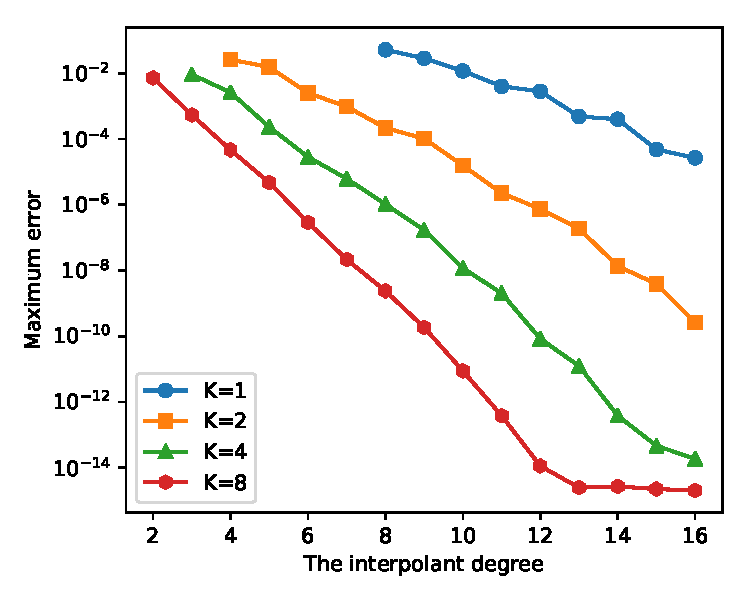
\includegraphics{tex/figures/interpolant_error}
	\fautor
	\label{fig:interpolant_error}
\end{figure}

\begin{figure}
	\centering
	\caption{The interpolation error measured on roots that were found after three Newton's iterations.}
	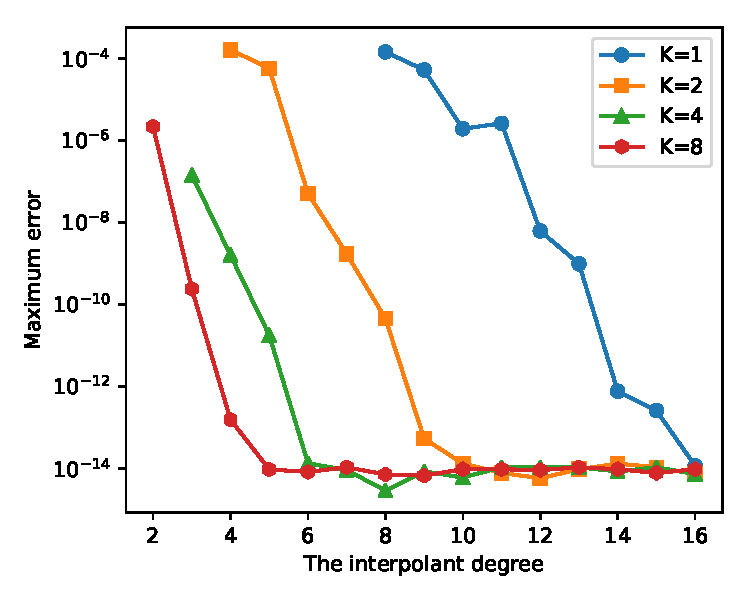
\includegraphics{tex/figures/interpolant_error_after_newton}
	\fautor
	\label{fig:interpolant_error_after_newton}
\end{figure}
